% Options for packages loaded elsewhere
\PassOptionsToPackage{unicode}{hyperref}
\PassOptionsToPackage{hyphens}{url}
\documentclass[
  spanish,
]{article}
\usepackage{xcolor}
\usepackage[margin=1in]{geometry}
\usepackage{amsmath,amssymb}
\setcounter{secnumdepth}{-\maxdimen} % remove section numbering
\usepackage{iftex}
\ifPDFTeX
  \usepackage[T1]{fontenc}
  \usepackage[utf8]{inputenc}
  \usepackage{textcomp} % provide euro and other symbols
\else % if luatex or xetex
  \usepackage{unicode-math} % this also loads fontspec
  \defaultfontfeatures{Scale=MatchLowercase}
  \defaultfontfeatures[\rmfamily]{Ligatures=TeX,Scale=1}
\fi
\usepackage{lmodern}
\ifPDFTeX\else
  % xetex/luatex font selection
\fi
% Use upquote if available, for straight quotes in verbatim environments
\IfFileExists{upquote.sty}{\usepackage{upquote}}{}
\IfFileExists{microtype.sty}{% use microtype if available
  \usepackage[]{microtype}
  \UseMicrotypeSet[protrusion]{basicmath} % disable protrusion for tt fonts
}{}
\makeatletter
\@ifundefined{KOMAClassName}{% if non-KOMA class
  \IfFileExists{parskip.sty}{%
    \usepackage{parskip}
  }{% else
    \setlength{\parindent}{0pt}
    \setlength{\parskip}{6pt plus 2pt minus 1pt}}
}{% if KOMA class
  \KOMAoptions{parskip=half}}
\makeatother
\usepackage{color}
\usepackage{fancyvrb}
\newcommand{\VerbBar}{|}
\newcommand{\VERB}{\Verb[commandchars=\\\{\}]}
\DefineVerbatimEnvironment{Highlighting}{Verbatim}{commandchars=\\\{\}}
% Add ',fontsize=\small' for more characters per line
\newenvironment{Shaded}{}{}
\newcommand{\AlertTok}[1]{\textcolor[rgb]{1.00,0.00,0.00}{\textbf{#1}}}
\newcommand{\AnnotationTok}[1]{\textcolor[rgb]{0.38,0.63,0.69}{\textbf{\textit{#1}}}}
\newcommand{\AttributeTok}[1]{\textcolor[rgb]{0.49,0.56,0.16}{#1}}
\newcommand{\BaseNTok}[1]{\textcolor[rgb]{0.25,0.63,0.44}{#1}}
\newcommand{\BuiltInTok}[1]{\textcolor[rgb]{0.00,0.50,0.00}{#1}}
\newcommand{\CharTok}[1]{\textcolor[rgb]{0.25,0.44,0.63}{#1}}
\newcommand{\CommentTok}[1]{\textcolor[rgb]{0.38,0.63,0.69}{\textit{#1}}}
\newcommand{\CommentVarTok}[1]{\textcolor[rgb]{0.38,0.63,0.69}{\textbf{\textit{#1}}}}
\newcommand{\ConstantTok}[1]{\textcolor[rgb]{0.53,0.00,0.00}{#1}}
\newcommand{\ControlFlowTok}[1]{\textcolor[rgb]{0.00,0.44,0.13}{\textbf{#1}}}
\newcommand{\DataTypeTok}[1]{\textcolor[rgb]{0.56,0.13,0.00}{#1}}
\newcommand{\DecValTok}[1]{\textcolor[rgb]{0.25,0.63,0.44}{#1}}
\newcommand{\DocumentationTok}[1]{\textcolor[rgb]{0.73,0.13,0.13}{\textit{#1}}}
\newcommand{\ErrorTok}[1]{\textcolor[rgb]{1.00,0.00,0.00}{\textbf{#1}}}
\newcommand{\ExtensionTok}[1]{#1}
\newcommand{\FloatTok}[1]{\textcolor[rgb]{0.25,0.63,0.44}{#1}}
\newcommand{\FunctionTok}[1]{\textcolor[rgb]{0.02,0.16,0.49}{#1}}
\newcommand{\ImportTok}[1]{\textcolor[rgb]{0.00,0.50,0.00}{\textbf{#1}}}
\newcommand{\InformationTok}[1]{\textcolor[rgb]{0.38,0.63,0.69}{\textbf{\textit{#1}}}}
\newcommand{\KeywordTok}[1]{\textcolor[rgb]{0.00,0.44,0.13}{\textbf{#1}}}
\newcommand{\NormalTok}[1]{#1}
\newcommand{\OperatorTok}[1]{\textcolor[rgb]{0.40,0.40,0.40}{#1}}
\newcommand{\OtherTok}[1]{\textcolor[rgb]{0.00,0.44,0.13}{#1}}
\newcommand{\PreprocessorTok}[1]{\textcolor[rgb]{0.74,0.48,0.00}{#1}}
\newcommand{\RegionMarkerTok}[1]{#1}
\newcommand{\SpecialCharTok}[1]{\textcolor[rgb]{0.25,0.44,0.63}{#1}}
\newcommand{\SpecialStringTok}[1]{\textcolor[rgb]{0.73,0.40,0.53}{#1}}
\newcommand{\StringTok}[1]{\textcolor[rgb]{0.25,0.44,0.63}{#1}}
\newcommand{\VariableTok}[1]{\textcolor[rgb]{0.10,0.09,0.49}{#1}}
\newcommand{\VerbatimStringTok}[1]{\textcolor[rgb]{0.25,0.44,0.63}{#1}}
\newcommand{\WarningTok}[1]{\textcolor[rgb]{0.38,0.63,0.69}{\textbf{\textit{#1}}}}
\usepackage{longtable,booktabs,array}
\newcounter{none} % for unnumbered tables
\usepackage{calc} % for calculating minipage widths
% Correct order of tables after \paragraph or \subparagraph
\usepackage{etoolbox}
\makeatletter
\patchcmd\longtable{\par}{\if@noskipsec\mbox{}\fi\par}{}{}
\makeatother
% Allow footnotes in longtable head/foot
\IfFileExists{footnotehyper.sty}{\usepackage{footnotehyper}}{\usepackage{footnote}}
\makesavenoteenv{longtable}
\usepackage{graphicx}
\makeatletter
\newsavebox\pandoc@box
\newcommand*\pandocbounded[1]{% scales image to fit in text height/width
  \sbox\pandoc@box{#1}%
  \Gscale@div\@tempa{\textheight}{\dimexpr\ht\pandoc@box+\dp\pandoc@box\relax}%
  \Gscale@div\@tempb{\linewidth}{\wd\pandoc@box}%
  \ifdim\@tempb\p@<\@tempa\p@\let\@tempa\@tempb\fi% select the smaller of both
  \ifdim\@tempa\p@<\p@\scalebox{\@tempa}{\usebox\pandoc@box}%
  \else\usebox{\pandoc@box}%
  \fi%
}
% Set default figure placement to htbp
\def\fps@figure{htbp}
\makeatother
\ifLuaTeX
\usepackage[bidi=basic,shorthands=off]{babel}
\else
\usepackage[bidi=default,shorthands=off]{babel}
\fi
\ifLuaTeX
  \usepackage{selnolig} % disable illegal ligatures
\fi
\setlength{\emergencystretch}{3em} % prevent overfull lines
\providecommand{\tightlist}{%
  \setlength{\itemsep}{0pt}\setlength{\parskip}{0pt}}
\usepackage{bookmark}
\IfFileExists{xurl.sty}{\usepackage{xurl}}{} % add URL line breaks if available
\urlstyle{same}
% fallback for those not using the hyperref driver hyperxmp:
\makeatletter
\@ifundefined{xmpquote}{\newcommand{\xmpquote}[1]{#1}}{}
\makeatother
\hypersetup{
  pdflang={es},
  hidelinks,
  pdfcreator={LaTeX via pandoc}}

\author{}
\date{}

\begin{document}

{
\setcounter{tocdepth}{3}
\tableofcontents
}
\section{Laboratorio: Hilos en Linux con
GCC}\label{laboratorio-hilos-en-linux-con-gcc}

\textbf{Plataforma:} GNU/Linux (Ubuntu / Debian)\\
\textbf{Compilador:} GCC\\
\textbf{Referencias:} - Tanenbaum \& Bos, \emph{Modern Operating
Systems}, 4.ª Ed., Sección 2.2 - Stallings, \emph{Operating Systems:
Internals and Design Principles}, 9.ª Ed., Cap. 4 (esp.~4.6)

\subsection{Contenido}\label{contenido}

\begin{itemize}
\tightlist
\item
  \hyperref[objetivo]{Objetivo}
\item
  \hyperref[preparaciuxf3n-del-entorno]{Preparación del entorno}

  \begin{itemize}
  \tightlist
  \item
    \hyperref[referencia-ruxe1pida-de-comandos]{Referencia rápida de
    comandos}
  \end{itemize}
\item
  \hyperref[ejercicio-1--identificaciuxf3n-de-un-hilo]{Ejercicio 1 ---
  Identificación de un hilo}
\item
  \hyperref[ejercicio-2--creaciuxf3n-de-hilos-con-pthread_create]{Ejercicio
  2 --- Creación de hilos con \texttt{pthread\_create()}}
\item
  \hyperref[ejercicio-3--memoria-compartida-y-condiciuxf3n-de-carrera]{Ejercicio
  3 --- Memoria compartida y condición de carrera}
\item
  \hyperref[ejercicio-4--estados-de-un-hilo-en-linux]{Ejercicio 4 ---
  Estados de un hilo en Linux}
\item
  \hyperref[ejercicio-5--task_struct-proceso-vs-hilo-en-linux]{Ejercicio
  5 --- \texttt{task\_struct}: proceso vs.~hilo en Linux}
\item
  \hyperref[ejercicio-6--hilos-en-el-sistema-exploraciuxf3n-con-herramientas]{Ejercicio
  6 --- Hilos en el sistema: exploración con herramientas}
\end{itemize}

\subsection{Objetivo}\label{objetivo}

Observar en Linux los conceptos teóricos de los Capítulos relacionados
con hilos y procesos, y cómo se implementan en la práctica:

\begin{itemize}
\tightlist
\item
  Identificación de hilos: TID de kernel vs.~identificador POSIX
\item
  Creación de hilos dentro de un proceso (\texttt{pthread\_create})
\item
  Memoria compartida y condición de carrera
\item
  Estados de un hilo (\texttt{R}, \texttt{S}, \texttt{D}, \texttt{T},
  \texttt{Z}) vistos en \texttt{/proc}
\item
  \texttt{task\_struct} y TGID: cómo Linux representa proceso vs.~hilo
\item
  Exploración de los hilos del sistema con herramientas estándar
\end{itemize}

\begin{center}\rule{0.5\linewidth}{0.5pt}\end{center}

\subsection{Preparación del entorno}\label{preparaciuxf3n-del-entorno}

\subsubsection{Instalar herramientas
necesarias}\label{instalar-herramientas-necesarias}

\begin{Shaded}
\begin{Highlighting}[]
\FunctionTok{sudo}\NormalTok{ apt update }\KeywordTok{\&\&} \FunctionTok{sudo}\NormalTok{ apt install }\AttributeTok{{-}y}\NormalTok{ gcc strace htop}
\end{Highlighting}
\end{Shaded}

{\def\LTcaptype{none} % do not increment counter
\begin{longtable}[]{@{}lll@{}}
\toprule\noalign{}
Paquete & Herramienta & Uso en el laboratorio \\
\midrule\noalign{}
\endhead
\bottomrule\noalign{}
\endlastfoot
\texttt{gcc} & compilador C & compilar todos los ejercicios \\
\texttt{strace} & \texttt{strace} & trazar la syscall \texttt{clone}
(ejercicio 2) \\
\texttt{htop} & \texttt{htop} & monitorear hilos del proceso en tiempo
real \\
\end{longtable}
}

Verifica la instalación:

\begin{Shaded}
\begin{Highlighting}[]
\FunctionTok{gcc} \AttributeTok{{-}{-}version} \KeywordTok{\&\&} \ExtensionTok{strace} \AttributeTok{{-}{-}version} \KeywordTok{\&\&} \ExtensionTok{htop} \AttributeTok{{-}{-}version}
\end{Highlighting}
\end{Shaded}

\begin{quote}
\textbf{Nota:} la biblioteca POSIX de hilos (\texttt{pthreads}) está
incluida en \texttt{glibc}. Solo se necesita el flag \texttt{-lpthread}
al compilar --- no hay paquete adicional.
\end{quote}

\subsubsection{Lanzar programas en segundo
plano}\label{lanzar-programas-en-segundo-plano}

El patrón \texttt{\&} + \texttt{\$!} permite observar el proceso desde
la misma terminal:

\begin{Shaded}
\begin{Highlighting}[]
\ExtensionTok{./programa} \KeywordTok{\&}
\VariableTok{PID}\OperatorTok{=}\VariableTok{$!}
\FunctionTok{sleep}\NormalTok{ 0.5}
\FunctionTok{ls}\NormalTok{ /proc/}\VariableTok{$PID}\NormalTok{/task          }\CommentTok{\# lista los hilos del proceso}
\end{Highlighting}
\end{Shaded}

\subsubsection{Referencia rápida de
comandos}\label{referencia-ruxe1pida-de-comandos}

\paragraph{Compilación con GCC y
pthreads}\label{compilaciuxf3n-con-gcc-y-pthreads}

{\def\LTcaptype{none} % do not increment counter
\begin{longtable}[]{@{}
  >{\raggedright\arraybackslash}p{(\linewidth - 2\tabcolsep) * \real{0.4091}}
  >{\raggedright\arraybackslash}p{(\linewidth - 2\tabcolsep) * \real{0.5909}}@{}}
\toprule\noalign{}
\begin{minipage}[b]{\linewidth}\raggedright
Comando
\end{minipage} & \begin{minipage}[b]{\linewidth}\raggedright
Descripción
\end{minipage} \\
\midrule\noalign{}
\endhead
\bottomrule\noalign{}
\endlastfoot
\texttt{gcc\ -Wall\ -pthread\ -o\ salida\ fuente.c} & Compila con
soporte POSIX threads; \texttt{-pthread} activa la biblioteca y los
flags del preprocesador necesarios \\
\texttt{./programa} & Ejecuta el binario en el directorio actual \\
\end{longtable}
}

\paragraph{Inspección de hilos}\label{inspecciuxf3n-de-hilos}

{\def\LTcaptype{none} % do not increment counter
\begin{longtable}[]{@{}
  >{\raggedright\arraybackslash}p{(\linewidth - 2\tabcolsep) * \real{0.4091}}
  >{\raggedright\arraybackslash}p{(\linewidth - 2\tabcolsep) * \real{0.5909}}@{}}
\toprule\noalign{}
\begin{minipage}[b]{\linewidth}\raggedright
Comando
\end{minipage} & \begin{minipage}[b]{\linewidth}\raggedright
Descripción
\end{minipage} \\
\midrule\noalign{}
\endhead
\bottomrule\noalign{}
\endlastfoot
\texttt{ls\ /proc/\textless{}PID\textgreater{}/task/} & Lista los TIDs
(kernel) de todos los hilos del proceso \\
\texttt{cat\ /proc/\textless{}PID\textgreater{}/task/\textless{}TID\textgreater{}/status}
& Estado del hilo individual (nombre, TID, estado) \\
\texttt{cat\ /proc/\textless{}PID\textgreater{}/task/\textless{}TID\textgreater{}/status\ \textbackslash{}\textbar{}\ grep\ State}
& Filtra solo el estado del hilo \\
\texttt{ps\ -p\ \textless{}PID\textgreater{}\ -L\ -o\ pid,lwp,state,comm}
& Lista hilos del proceso con sus LWPs y estados \\
\end{longtable}
}

\paragraph{Herramientas de monitoreo}\label{herramientas-de-monitoreo}

{\def\LTcaptype{none} % do not increment counter
\begin{longtable}[]{@{}
  >{\raggedright\arraybackslash}p{(\linewidth - 2\tabcolsep) * \real{0.4091}}
  >{\raggedright\arraybackslash}p{(\linewidth - 2\tabcolsep) * \real{0.5909}}@{}}
\toprule\noalign{}
\begin{minipage}[b]{\linewidth}\raggedright
Comando
\end{minipage} & \begin{minipage}[b]{\linewidth}\raggedright
Descripción
\end{minipage} \\
\midrule\noalign{}
\endhead
\bottomrule\noalign{}
\endlastfoot
\texttt{strace\ -e\ trace=clone\ ./prog} & Muestra la llamada
\texttt{clone()} que crea cada hilo \\
\texttt{htop} & Monitor interactivo; presiona \texttt{H} para ver hilos
individuales dentro de cada proceso \\
\end{longtable}
}

\paragraph{\texorpdfstring{Estados de hilo en
\texttt{/proc}}{Estados de hilo en /proc}}\label{estados-de-hilo-en-proc}

{\def\LTcaptype{none} % do not increment counter
\begin{longtable}[]{@{}lll@{}}
\toprule\noalign{}
Letra & Estado & Significado \\
\midrule\noalign{}
\endhead
\bottomrule\noalign{}
\endlastfoot
\texttt{R} & Running / Runnable & En CPU o listo en la cola \\
\texttt{S} & Sleeping & Bloqueado (esperando mutex, E/S, join\ldots) \\
\texttt{Z} & Zombie & El hilo terminó y aún no fue recogido \\
\end{longtable}
}

\begin{center}\rule{0.5\linewidth}{0.5pt}\end{center}

\subsubsection{Directorio de trabajo}\label{directorio-de-trabajo}

\begin{Shaded}
\begin{Highlighting}[]
\FunctionTok{mkdir}\NormalTok{ \textasciitilde{}/lab{-}hilos}
\BuiltInTok{cd}\NormalTok{ \textasciitilde{}/lab{-}hilos}
\end{Highlighting}
\end{Shaded}

\subsubsection{Script de compilación
rápida}\label{script-de-compilaciuxf3n-ruxe1pida}

Guarda como \texttt{run.sh}:

\begin{Shaded}
\begin{Highlighting}[]
\CommentTok{\#!/bin/bash}
\CommentTok{\# Uso: bash run.sh nombre\_sin\_extension}
\FunctionTok{gcc} \AttributeTok{{-}Wall} \AttributeTok{{-}pthread} \AttributeTok{{-}o} \StringTok{"}\VariableTok{$1}\StringTok{"} \StringTok{"}\VariableTok{$1}\StringTok{.c"} \KeywordTok{\&\&} \ExtensionTok{./}\StringTok{"}\VariableTok{$1}\StringTok{"}
\end{Highlighting}
\end{Shaded}

\begin{Shaded}
\begin{Highlighting}[]
\FunctionTok{chmod}\NormalTok{ +x run.sh}
\end{Highlighting}
\end{Shaded}

\begin{center}\rule{0.5\linewidth}{0.5pt}\end{center}

\subsection{Ejercicio 1 --- Identificación de un
hilo}\label{ejercicio-1-identificaciuxf3n-de-un-hilo}

\subsubsection{Conceptos relacionados}\label{conceptos-relacionados}

En Linux cada hilo es un \texttt{task\_struct} con su propio \textbf{TID
de kernel} (visible en \texttt{/proc}). La API POSIX expone un
identificador opaco \texttt{pthread\_t} (retornado por
\texttt{pthread\_self()}). El proceso padre sigue siendo el mismo para
todos los hilos (mismo \texttt{getpid()}).

{\def\LTcaptype{none} % do not increment counter
\begin{longtable}[]{@{}
  >{\raggedright\arraybackslash}p{(\linewidth - 6\tabcolsep) * \real{0.1522}}
  >{\raggedright\arraybackslash}p{(\linewidth - 6\tabcolsep) * \real{0.1957}}
  >{\raggedright\arraybackslash}p{(\linewidth - 6\tabcolsep) * \real{0.2174}}
  >{\raggedright\arraybackslash}p{(\linewidth - 6\tabcolsep) * \real{0.4348}}@{}}
\toprule\noalign{}
\begin{minipage}[b]{\linewidth}\raggedright
Campo
\end{minipage} & \begin{minipage}[b]{\linewidth}\raggedright
Función
\end{minipage} & \begin{minipage}[b]{\linewidth}\raggedright
API en C
\end{minipage} & \begin{minipage}[b]{\linewidth}\raggedright
Visible en \texttt{/proc}
\end{minipage} \\
\midrule\noalign{}
\endhead
\bottomrule\noalign{}
\endlastfoot
\textbf{PID del proceso} & Identifica al proceso dueño de todos los
hilos & \texttt{getpid()} &
\texttt{/proc/\textless{}PID\textgreater{}/} \\
\textbf{TID de kernel} & Identifica al hilo individual dentro del kernel
& \texttt{gettid()} \emph{(Linux 2.4.11+)} &
\texttt{/proc/\textless{}PID\textgreater{}/task/\textless{}TID\textgreater{}/} \\
\textbf{pthread\_t} & Identificador opaco POSIX del hilo &
\texttt{pthread\_self()} & --- \\
\end{longtable}
}

\subsubsection{\texorpdfstring{Código ---
\texttt{t1\_identidad.c}}{Código --- t1\_identidad.c}}\label{cuxf3digo-t1_identidad.c}

\begin{Shaded}
\begin{Highlighting}[]
\PreprocessorTok{\#define }\OtherTok{\_GNU\_SOURCE}
\PreprocessorTok{\#include }\ImportTok{\textless{}stdio.h\textgreater{}}
\PreprocessorTok{\#include }\ImportTok{\textless{}unistd.h\textgreater{}}
\PreprocessorTok{\#include }\ImportTok{\textless{}pthread.h\textgreater{}}

\DataTypeTok{static} \DataTypeTok{void} \OperatorTok{*}\NormalTok{funcion\_hilo}\OperatorTok{(}\DataTypeTok{void} \OperatorTok{*}\NormalTok{arg}\OperatorTok{)} \OperatorTok{\{}
    \DataTypeTok{int}\NormalTok{ numero }\OperatorTok{=} \OperatorTok{*(}\DataTypeTok{int} \OperatorTok{*)}\NormalTok{arg}\OperatorTok{;}
\NormalTok{    printf}\OperatorTok{(}\StringTok{"[hilo }\SpecialCharTok{\%d}\StringTok{] pthread\_self = }\SpecialCharTok{\%lu}\StringTok{  gettid = }\SpecialCharTok{\%d}\StringTok{  getpid = }\SpecialCharTok{\%d\textbackslash{}n}\StringTok{"}\OperatorTok{,}
\NormalTok{           numero}\OperatorTok{,} \OperatorTok{(}\DataTypeTok{unsigned} \DataTypeTok{long}\OperatorTok{)}\NormalTok{pthread\_self}\OperatorTok{(),}\NormalTok{ gettid}\OperatorTok{(),}\NormalTok{ getpid}\OperatorTok{());}
    \ControlFlowTok{return}\NormalTok{ NULL}\OperatorTok{;}
\OperatorTok{\}}

\DataTypeTok{int}\NormalTok{ main}\OperatorTok{(}\DataTypeTok{void}\OperatorTok{)} \OperatorTok{\{}
\NormalTok{    pthread\_t h1}\OperatorTok{,}\NormalTok{ h2}\OperatorTok{;}
    \DataTypeTok{int}\NormalTok{ n1 }\OperatorTok{=} \DecValTok{1}\OperatorTok{,}\NormalTok{ n2 }\OperatorTok{=} \DecValTok{2}\OperatorTok{;}

\NormalTok{    printf}\OperatorTok{(}\StringTok{"[main]   pthread\_self = }\SpecialCharTok{\%lu}\StringTok{  gettid = }\SpecialCharTok{\%d}\StringTok{  getpid = }\SpecialCharTok{\%d\textbackslash{}n}\StringTok{"}\OperatorTok{,}
           \OperatorTok{(}\DataTypeTok{unsigned} \DataTypeTok{long}\OperatorTok{)}\NormalTok{pthread\_self}\OperatorTok{(),}\NormalTok{ gettid}\OperatorTok{(),}\NormalTok{ getpid}\OperatorTok{());}

\NormalTok{    pthread\_create}\OperatorTok{(\&}\NormalTok{h1}\OperatorTok{,}\NormalTok{ NULL}\OperatorTok{,}\NormalTok{ funcion\_hilo}\OperatorTok{,} \OperatorTok{\&}\NormalTok{n1}\OperatorTok{);}
\NormalTok{    pthread\_create}\OperatorTok{(\&}\NormalTok{h2}\OperatorTok{,}\NormalTok{ NULL}\OperatorTok{,}\NormalTok{ funcion\_hilo}\OperatorTok{,} \OperatorTok{\&}\NormalTok{n2}\OperatorTok{);}

\NormalTok{    pthread\_join}\OperatorTok{(}\NormalTok{h1}\OperatorTok{,}\NormalTok{ NULL}\OperatorTok{);}
\NormalTok{    pthread\_join}\OperatorTok{(}\NormalTok{h2}\OperatorTok{,}\NormalTok{ NULL}\OperatorTok{);}
    \ControlFlowTok{return} \DecValTok{0}\OperatorTok{;}
\OperatorTok{\}}
\end{Highlighting}
\end{Shaded}

\subsubsection{Compilación y
ejecución}\label{compilaciuxf3n-y-ejecuciuxf3n}

\begin{Shaded}
\begin{Highlighting}[]
\FunctionTok{gcc} \AttributeTok{{-}Wall} \AttributeTok{{-}pthread} \AttributeTok{{-}o}\NormalTok{ t1\_identidad t1\_identidad.c}
\ExtensionTok{./t1\_identidad}
\end{Highlighting}
\end{Shaded}

\subsubsection{\texorpdfstring{Observación con
\texttt{/proc}}{Observación con /proc}}\label{observaciuxf3n-con-proc}

\begin{Shaded}
\begin{Highlighting}[]
\ExtensionTok{./t1\_identidad} \KeywordTok{\&}
\VariableTok{PID}\OperatorTok{=}\VariableTok{$!}
\FunctionTok{sleep}\NormalTok{ 0.1}
\FunctionTok{ls}\NormalTok{ /proc/}\VariableTok{$PID}\NormalTok{/task}
\CommentTok{\# muestra tres TIDs: el hilo principal + dos hilos creados}
\end{Highlighting}
\end{Shaded}

\subsubsection{Salida esperada}\label{salida-esperada}

\begin{verbatim}
[main]   pthread_self = 139...  gettid = 4210  getpid = 4210
[hilo 1] pthread_self = 139...  gettid = 4211  getpid = 4210
[hilo 2] pthread_self = 139...  gettid = 4212  getpid = 4210
\end{verbatim}

\subsubsection{Preguntas de análisis}\label{preguntas-de-anuxe1lisis}

\begin{enumerate}
\def\labelenumi{\arabic{enumi}.}
\tightlist
\item
  ¿Por qué \texttt{getpid()} devuelve el mismo valor en el hilo
  principal y en los hilos creados?
\item
  El TID del hilo principal coincide con el PID del proceso. Explica por
  qué usando lo que sabes de \texttt{task\_struct} en Linux.
\item
  ¿Qué diferencia hay entre \texttt{pthread\_t} y el TID de kernel?
\end{enumerate}

\begin{center}\rule{0.5\linewidth}{0.5pt}\end{center}

\subsection{\texorpdfstring{Ejercicio 2 --- Creación de hilos con
\texttt{pthread\_create()}}{Ejercicio 2 --- Creación de hilos con pthread\_create()}}\label{ejercicio-2-creaciuxf3n-de-hilos-con-pthread_create}

\subsubsection{Conceptos relacionados}\label{conceptos-relacionados-1}

\texttt{pthread\_create()} crea un nuevo hilo de ejecución dentro del
\textbf{mismo proceso}. Internamente invoca la syscall \texttt{clone()}
con flags que permiten compartir espacio de memoria, descriptores de
archivo y señales:

\begin{figure}
\centering
\pandocbounded{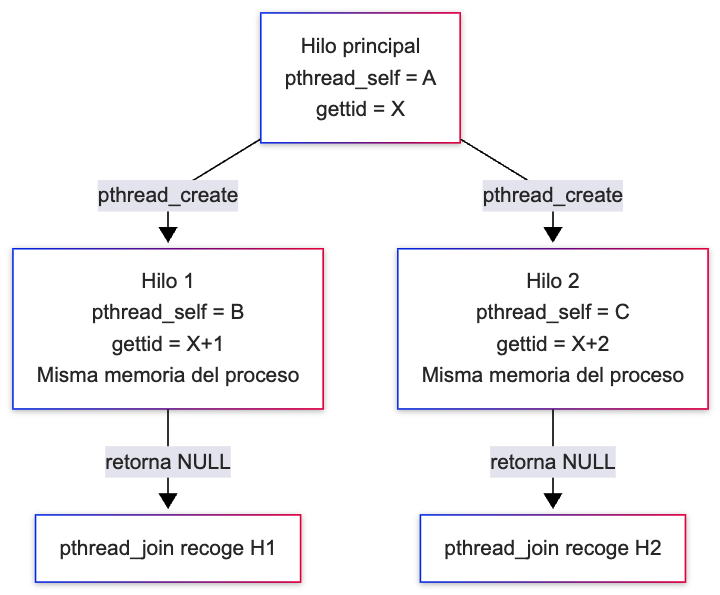
\includegraphics[keepaspectratio,alt={Diagrama de creación de hilos}]{img/thread_management_linux.png}}
\caption{Diagrama de creación de hilos}
\end{figure}

\begin{quote}
\textbf{Diferencia con \texttt{fork()}:} \texttt{fork()} copia el
espacio de direcciones (o usa COW); \texttt{pthread\_create()} comparte
el mismo espacio. Un hilo nuevo es más barato de crear y puede
comunicarse directamente a través de variables globales.
\end{quote}

\subsubsection{\texorpdfstring{Código ---
\texttt{t2\_create.c}}{Código --- t2\_create.c}}\label{cuxf3digo-t2_create.c}

\begin{Shaded}
\begin{Highlighting}[]
\PreprocessorTok{\#include }\ImportTok{\textless{}stdio.h\textgreater{}}
\PreprocessorTok{\#include }\ImportTok{\textless{}unistd.h\textgreater{}}
\PreprocessorTok{\#include }\ImportTok{\textless{}pthread.h\textgreater{}}

\DataTypeTok{static} \DataTypeTok{void} \OperatorTok{*}\NormalTok{tarea}\OperatorTok{(}\DataTypeTok{void} \OperatorTok{*}\NormalTok{arg}\OperatorTok{)} \OperatorTok{\{}
    \DataTypeTok{int}\NormalTok{ id }\OperatorTok{=} \OperatorTok{*(}\DataTypeTok{int} \OperatorTok{*)}\NormalTok{arg}\OperatorTok{;}
\NormalTok{    printf}\OperatorTok{(}\StringTok{"[hilo }\SpecialCharTok{\%d}\StringTok{] inicio — ejecutando concurrentemente con main}\SpecialCharTok{\textbackslash{}n}\StringTok{"}\OperatorTok{,}\NormalTok{ id}\OperatorTok{);}
\NormalTok{    sleep}\OperatorTok{(}\DecValTok{1}\OperatorTok{);}
\NormalTok{    printf}\OperatorTok{(}\StringTok{"[hilo }\SpecialCharTok{\%d}\StringTok{] fin}\SpecialCharTok{\textbackslash{}n}\StringTok{"}\OperatorTok{,}\NormalTok{ id}\OperatorTok{);}
    \ControlFlowTok{return}\NormalTok{ NULL}\OperatorTok{;}
\OperatorTok{\}}

\DataTypeTok{int}\NormalTok{ main}\OperatorTok{(}\DataTypeTok{void}\OperatorTok{)} \OperatorTok{\{}
\NormalTok{    pthread\_t hilos}\OperatorTok{[}\DecValTok{3}\OperatorTok{];}
    \DataTypeTok{int}\NormalTok{ ids}\OperatorTok{[}\DecValTok{3}\OperatorTok{]} \OperatorTok{=} \OperatorTok{\{}\DecValTok{1}\OperatorTok{,} \DecValTok{2}\OperatorTok{,} \DecValTok{3}\OperatorTok{\};}

\NormalTok{    printf}\OperatorTok{(}\StringTok{"[main] creando 3 hilos...}\SpecialCharTok{\textbackslash{}n}\StringTok{"}\OperatorTok{);}
    \ControlFlowTok{for} \OperatorTok{(}\DataTypeTok{int}\NormalTok{ i }\OperatorTok{=} \DecValTok{0}\OperatorTok{;}\NormalTok{ i }\OperatorTok{\textless{}} \DecValTok{3}\OperatorTok{;}\NormalTok{ i}\OperatorTok{++)}
\NormalTok{        pthread\_create}\OperatorTok{(\&}\NormalTok{hilos}\OperatorTok{[}\NormalTok{i}\OperatorTok{],}\NormalTok{ NULL}\OperatorTok{,}\NormalTok{ tarea}\OperatorTok{,} \OperatorTok{\&}\NormalTok{ids}\OperatorTok{[}\NormalTok{i}\OperatorTok{]);}

\NormalTok{    printf}\OperatorTok{(}\StringTok{"[main] hilos creados, esperando con join...}\SpecialCharTok{\textbackslash{}n}\StringTok{"}\OperatorTok{);}
    \ControlFlowTok{for} \OperatorTok{(}\DataTypeTok{int}\NormalTok{ i }\OperatorTok{=} \DecValTok{0}\OperatorTok{;}\NormalTok{ i }\OperatorTok{\textless{}} \DecValTok{3}\OperatorTok{;}\NormalTok{ i}\OperatorTok{++)}
\NormalTok{        pthread\_join}\OperatorTok{(}\NormalTok{hilos}\OperatorTok{[}\NormalTok{i}\OperatorTok{],}\NormalTok{ NULL}\OperatorTok{);}

\NormalTok{    printf}\OperatorTok{(}\StringTok{"[main] todos los hilos terminaron}\SpecialCharTok{\textbackslash{}n}\StringTok{"}\OperatorTok{);}
    \ControlFlowTok{return} \DecValTok{0}\OperatorTok{;}
\OperatorTok{\}}
\end{Highlighting}
\end{Shaded}

\subsubsection{Compilación y
ejecución}\label{compilaciuxf3n-y-ejecuciuxf3n-1}

\begin{Shaded}
\begin{Highlighting}[]
\FunctionTok{gcc} \AttributeTok{{-}Wall} \AttributeTok{{-}pthread} \AttributeTok{{-}o}\NormalTok{ t2\_create t2\_create.c}
\ExtensionTok{./t2\_create}
\end{Highlighting}
\end{Shaded}

\subsubsection{\texorpdfstring{Trazado con
\texttt{strace}}{Trazado con strace}}\label{trazado-con-strace}

\begin{Shaded}
\begin{Highlighting}[]
\ExtensionTok{strace} \AttributeTok{{-}e}\NormalTok{ trace=clone ./t2\_create }\DecValTok{2}\OperatorTok{\textgreater{}\&}\DecValTok{1} \KeywordTok{|} \FunctionTok{grep}\NormalTok{ clone}
\end{Highlighting}
\end{Shaded}

Cada llamada a \texttt{pthread\_create()} genera un \texttt{clone()} con
flags como \texttt{CLONE\_VM}, \texttt{CLONE\_FILES},
\texttt{CLONE\_THREAD}, \texttt{CLONE\_SIGHAND}.

\subsubsection{Salida esperada}\label{salida-esperada-1}

\begin{verbatim}
[main] creando 3 hilos...
[main] hilos creados, esperando con join...
[hilo 1] inicio — ejecutando concurrentemente con main
[hilo 2] inicio — ejecutando concurrentemente con main
[hilo 3] inicio — ejecutando concurrentemente con main
[hilo 1] fin
[hilo 2] fin
[hilo 3] fin
[main] todos los hilos terminaron
\end{verbatim}

\begin{quote}
El orden de los hilos puede variar entre ejecuciones --- el planificador
decide cuál ejecuta primero.
\end{quote}

\subsubsection{Preguntas de análisis}\label{preguntas-de-anuxe1lisis-1}

\begin{enumerate}
\def\labelenumi{\arabic{enumi}.}
\tightlist
\item
  Ejecuta el programa varias veces. ¿El orden de los mensajes
  \texttt{inicio} y \texttt{fin} es siempre el mismo? ¿Por qué?
\item
  En el \texttt{strace}, identifica los flags de \texttt{clone()}.
  ¿Cuáles indican que los hilos comparten memoria?
\item
  ¿Qué pasaría si llamaras a \texttt{fork()} en lugar de
  \texttt{pthread\_create()}? ¿Podrían los hijos comunicarse
  directamente a través de una variable global?
\end{enumerate}

\begin{center}\rule{0.5\linewidth}{0.5pt}\end{center}

\subsection{Ejercicio 3 --- Memoria compartida y condición de
carrera}\label{ejercicio-3-memoria-compartida-y-condiciuxf3n-de-carrera}

\subsubsection{Conceptos relacionados}\label{conceptos-relacionados-2}

Los hilos comparten el mismo espacio de direcciones, incluyendo
variables globales y del heap. Sin sincronización, cuando dos hilos leen
y modifican la misma variable de forma concurrente ocurre una
\textbf{condición de carrera} (\emph{race condition}): el resultado
depende del orden de ejecución --- no es determinista.

La secuencia problemática (ejemplo con \texttt{contador++}):

\begin{verbatim}
Hilo A lee contador = 100
Hilo B lee contador = 100       ← B lee ANTES de que A escriba
Hilo A escribe contador = 101
Hilo B escribe contador = 101   ← se pierde un incremento
\end{verbatim}

\subsubsection{\texorpdfstring{Código ---
\texttt{t3\_carrera.c}}{Código --- t3\_carrera.c}}\label{cuxf3digo-t3_carrera.c}

\begin{Shaded}
\begin{Highlighting}[]
\PreprocessorTok{\#include }\ImportTok{\textless{}stdio.h\textgreater{}}
\PreprocessorTok{\#include }\ImportTok{\textless{}pthread.h\textgreater{}}

\PreprocessorTok{\#define N\_HILOS    }\DecValTok{4}
\PreprocessorTok{\#define ITERACIONES }\DecValTok{1000000}

\DataTypeTok{static} \DataTypeTok{long}\NormalTok{ contador }\OperatorTok{=} \DecValTok{0}\OperatorTok{;}   \CommentTok{/* variable compartida — sin protección */}

\DataTypeTok{static} \DataTypeTok{void} \OperatorTok{*}\NormalTok{incrementar}\OperatorTok{(}\DataTypeTok{void} \OperatorTok{*}\NormalTok{arg}\OperatorTok{)} \OperatorTok{\{}
    \ControlFlowTok{for} \OperatorTok{(}\DataTypeTok{int}\NormalTok{ i }\OperatorTok{=} \DecValTok{0}\OperatorTok{;}\NormalTok{ i }\OperatorTok{\textless{}}\NormalTok{ ITERACIONES}\OperatorTok{;}\NormalTok{ i}\OperatorTok{++)}
\NormalTok{        contador}\OperatorTok{++;}          \CommentTok{/* lectura{-}modificación{-}escritura NO atómica */}
    \ControlFlowTok{return}\NormalTok{ NULL}\OperatorTok{;}
\OperatorTok{\}}

\DataTypeTok{int}\NormalTok{ main}\OperatorTok{(}\DataTypeTok{void}\OperatorTok{)} \OperatorTok{\{}
\NormalTok{    pthread\_t hilos}\OperatorTok{[}\NormalTok{N\_HILOS}\OperatorTok{];}

    \ControlFlowTok{for} \OperatorTok{(}\DataTypeTok{int}\NormalTok{ i }\OperatorTok{=} \DecValTok{0}\OperatorTok{;}\NormalTok{ i }\OperatorTok{\textless{}}\NormalTok{ N\_HILOS}\OperatorTok{;}\NormalTok{ i}\OperatorTok{++)}
\NormalTok{        pthread\_create}\OperatorTok{(\&}\NormalTok{hilos}\OperatorTok{[}\NormalTok{i}\OperatorTok{],}\NormalTok{ NULL}\OperatorTok{,}\NormalTok{ incrementar}\OperatorTok{,}\NormalTok{ NULL}\OperatorTok{);}

    \ControlFlowTok{for} \OperatorTok{(}\DataTypeTok{int}\NormalTok{ i }\OperatorTok{=} \DecValTok{0}\OperatorTok{;}\NormalTok{ i }\OperatorTok{\textless{}}\NormalTok{ N\_HILOS}\OperatorTok{;}\NormalTok{ i}\OperatorTok{++)}
\NormalTok{        pthread\_join}\OperatorTok{(}\NormalTok{hilos}\OperatorTok{[}\NormalTok{i}\OperatorTok{],}\NormalTok{ NULL}\OperatorTok{);}

\NormalTok{    printf}\OperatorTok{(}\StringTok{"Resultado: }\SpecialCharTok{\%ld}\StringTok{  (esperado: }\SpecialCharTok{\%d}\StringTok{)}\SpecialCharTok{\textbackslash{}n}\StringTok{"}\OperatorTok{,}
\NormalTok{           contador}\OperatorTok{,}\NormalTok{ N\_HILOS }\OperatorTok{*}\NormalTok{ ITERACIONES}\OperatorTok{);}
    \ControlFlowTok{return} \DecValTok{0}\OperatorTok{;}
\OperatorTok{\}}
\end{Highlighting}
\end{Shaded}

\subsubsection{Compilación y
ejecución}\label{compilaciuxf3n-y-ejecuciuxf3n-2}

\begin{Shaded}
\begin{Highlighting}[]
\FunctionTok{gcc} \AttributeTok{{-}Wall} \AttributeTok{{-}pthread} \AttributeTok{{-}o}\NormalTok{ t3\_carrera t3\_carrera.c}
\ExtensionTok{./t3\_carrera}
\ExtensionTok{./t3\_carrera}
\ExtensionTok{./t3\_carrera}
\end{Highlighting}
\end{Shaded}

\subsubsection{Salida esperada}\label{salida-esperada-2}

\begin{verbatim}
Resultado: 1843217  (esperado: 4000000)
Resultado: 2671004  (esperado: 4000000)
Resultado: 3102891  (esperado: 4000000)
\end{verbatim}

El resultado cambia en cada ejecución y es siempre menor que el esperado
--- evidencia directa de la condición de carrera.

\subsubsection{Preguntas de análisis}\label{preguntas-de-anuxe1lisis-2}

\begin{enumerate}
\def\labelenumi{\arabic{enumi}.}
\tightlist
\item
  ¿Por qué \texttt{contador++} no es una operación atómica? Descomponer
  la instrucción en pasos de CPU (leer, modificar, escribir).
\item
  ¿Por qué el resultado siempre es \emph{menor} que
  \texttt{N\_HILOS\ ×\ ITERACIONES} y nunca mayor?
\item
  ¿Qué ocurre si reduces \texttt{N\_HILOS} a 1? ¿Aparece la condición de
  carrera?
\end{enumerate}

\begin{center}\rule{0.5\linewidth}{0.5pt}\end{center}

\subsection{Ejercicio 4 --- Estados de un hilo en
Linux}\label{ejercicio-4-estados-de-un-hilo-en-linux}

\subsubsection{Conceptos relacionados}\label{conceptos-relacionados-3}

Linux no distingue estados de hilo de los de proceso: cada hilo es un
\texttt{task\_struct} y expone el mismo conjunto de estados en
\texttt{/proc/\textless{}PID\textgreater{}/task/\textless{}TID\textgreater{}/status}.

{\def\LTcaptype{none} % do not increment counter
\begin{longtable}[]{@{}
  >{\raggedright\arraybackslash}p{(\linewidth - 4\tabcolsep) * \real{0.2000}}
  >{\raggedright\arraybackslash}p{(\linewidth - 4\tabcolsep) * \real{0.4750}}
  >{\raggedright\arraybackslash}p{(\linewidth - 4\tabcolsep) * \real{0.3250}}@{}}
\toprule\noalign{}
\begin{minipage}[b]{\linewidth}\raggedright
Estado
\end{minipage} & \begin{minipage}[b]{\linewidth}\raggedright
Letra en \texttt{/proc}
\end{minipage} & \begin{minipage}[b]{\linewidth}\raggedright
Descripción
\end{minipage} \\
\midrule\noalign{}
\endhead
\bottomrule\noalign{}
\endlastfoot
\textbf{Running/Runnable} & \texttt{R} & En CPU o listo en la cola de
ejecución \\
\textbf{Sleeping (interruptible)} & \texttt{S} & Bloqueado esperando
E/S, señal, \texttt{sleep()}, mutex, etc. \\
\textbf{Uninterruptible sleep} & \texttt{D} & Esperando E/S de disco; no
puede interrumpirse con señales \\
\textbf{Stopped} & \texttt{T} & Detenido por \texttt{SIGSTOP} o being
traced (\texttt{ptrace}) \\
\textbf{Zombie} & \texttt{Z} & Terminó pero nadie ha hecho
\texttt{pthread\_join}/\texttt{wait} sobre él \\
\end{longtable}
}

\subsubsection{\texorpdfstring{Código ---
\texttt{t4\_estados.c}}{Código --- t4\_estados.c}}\label{cuxf3digo-t4_estados.c}

\begin{Shaded}
\begin{Highlighting}[]
\PreprocessorTok{\#include }\ImportTok{\textless{}stdio.h\textgreater{}}
\PreprocessorTok{\#include }\ImportTok{\textless{}unistd.h\textgreater{}}
\PreprocessorTok{\#include }\ImportTok{\textless{}pthread.h\textgreater{}}

\CommentTok{/* Demostración de estados de hilo: R (ocupado) y S (durmiendo). */}

\DataTypeTok{static} \DataTypeTok{void} \OperatorTok{*}\NormalTok{hilo\_ocupado}\OperatorTok{(}\DataTypeTok{void} \OperatorTok{*}\NormalTok{arg}\OperatorTok{)} \OperatorTok{\{}
\NormalTok{    printf}\OperatorTok{(}\StringTok{"[ocupado]  TID = }\SpecialCharTok{\%d}\StringTok{ — bucle intensivo (→ R)}\SpecialCharTok{\textbackslash{}n}\StringTok{"}\OperatorTok{,}\NormalTok{ gettid}\OperatorTok{());}
    \DataTypeTok{volatile} \DataTypeTok{long}\NormalTok{ suma }\OperatorTok{=} \DecValTok{0}\OperatorTok{;}
    \ControlFlowTok{for} \OperatorTok{(}\DataTypeTok{long}\NormalTok{ i }\OperatorTok{=} \DecValTok{0}\OperatorTok{;}\NormalTok{ i }\OperatorTok{\textless{}} \DecValTok{3000000000}\BuiltInTok{L}\OperatorTok{;}\NormalTok{ i}\OperatorTok{++)}
\NormalTok{        suma }\OperatorTok{+=}\NormalTok{ i}\OperatorTok{;}
\NormalTok{    printf}\OperatorTok{(}\StringTok{"[ocupado]  fin, suma = }\SpecialCharTok{\%ld\textbackslash{}n}\StringTok{"}\OperatorTok{,}\NormalTok{ suma}\OperatorTok{);}
    \ControlFlowTok{return}\NormalTok{ NULL}\OperatorTok{;}
\OperatorTok{\}}

\DataTypeTok{static} \DataTypeTok{void} \OperatorTok{*}\NormalTok{hilo\_durmiente}\OperatorTok{(}\DataTypeTok{void} \OperatorTok{*}\NormalTok{arg}\OperatorTok{)} \OperatorTok{\{}
\NormalTok{    printf}\OperatorTok{(}\StringTok{"[durmiente] TID = }\SpecialCharTok{\%d}\StringTok{ — sleep(4) (→ S)}\SpecialCharTok{\textbackslash{}n}\StringTok{"}\OperatorTok{,}\NormalTok{ gettid}\OperatorTok{());}
\NormalTok{    sleep}\OperatorTok{(}\DecValTok{4}\OperatorTok{);}
\NormalTok{    printf}\OperatorTok{(}\StringTok{"[durmiente] desperté (→ R)}\SpecialCharTok{\textbackslash{}n}\StringTok{"}\OperatorTok{);}
    \ControlFlowTok{return}\NormalTok{ NULL}\OperatorTok{;}
\OperatorTok{\}}

\DataTypeTok{int}\NormalTok{ main}\OperatorTok{(}\DataTypeTok{void}\OperatorTok{)} \OperatorTok{\{}
\NormalTok{    pthread\_t h1}\OperatorTok{,}\NormalTok{ h2}\OperatorTok{;}

\NormalTok{    printf}\OperatorTok{(}\StringTok{"[main] PID = }\SpecialCharTok{\%d\textbackslash{}n}\StringTok{"}\OperatorTok{,}\NormalTok{ getpid}\OperatorTok{());}
\NormalTok{    pthread\_create}\OperatorTok{(\&}\NormalTok{h1}\OperatorTok{,}\NormalTok{ NULL}\OperatorTok{,}\NormalTok{ hilo\_ocupado}\OperatorTok{,}\NormalTok{ NULL}\OperatorTok{);}
\NormalTok{    pthread\_create}\OperatorTok{(\&}\NormalTok{h2}\OperatorTok{,}\NormalTok{ NULL}\OperatorTok{,}\NormalTok{ hilo\_durmiente}\OperatorTok{,}\NormalTok{ NULL}\OperatorTok{);}

\NormalTok{    pthread\_join}\OperatorTok{(}\NormalTok{h1}\OperatorTok{,}\NormalTok{ NULL}\OperatorTok{);}
\NormalTok{    pthread\_join}\OperatorTok{(}\NormalTok{h2}\OperatorTok{,}\NormalTok{ NULL}\OperatorTok{);}
\NormalTok{    printf}\OperatorTok{(}\StringTok{"[main] ambos hilos terminaron}\SpecialCharTok{\textbackslash{}n}\StringTok{"}\OperatorTok{);}
    \ControlFlowTok{return} \DecValTok{0}\OperatorTok{;}
\OperatorTok{\}}
\end{Highlighting}
\end{Shaded}

\subsubsection{Compilación y
ejecución}\label{compilaciuxf3n-y-ejecuciuxf3n-3}

\begin{Shaded}
\begin{Highlighting}[]
\FunctionTok{gcc} \AttributeTok{{-}Wall} \AttributeTok{{-}pthread} \AttributeTok{{-}o}\NormalTok{ t4\_estados t4\_estados.c}
\ExtensionTok{./t4\_estados} \KeywordTok{\&}
\VariableTok{PID}\OperatorTok{=}\VariableTok{$!}
\FunctionTok{sleep}\NormalTok{ 1}
\FunctionTok{ps} \AttributeTok{{-}p} \VariableTok{$PID} \AttributeTok{{-}L} \AttributeTok{{-}o}\NormalTok{ pid,lwp,state,comm}
\CommentTok{\# uno de los LWP debería verse en R y el otro en S}
\end{Highlighting}
\end{Shaded}

\subsubsection{Salida esperada}\label{salida-esperada-3}

\begin{verbatim}
[main] PID = 8341
[ocupado]  TID = 8342 — bucle intensivo (→ R)
[durmiente] TID = 8343 — sleep(4) (→ S)
  PID   LWP S COMMAND
 8341  8341 S t4_estados
 8341  8342 R t4_estados
 8341  8343 S t4_estados
[durmiente] desperté (→ R)
[ocupado]  fin, suma = ...
[main] ambos hilos terminaron
\end{verbatim}

\subsubsection{Preguntas de análisis}\label{preguntas-de-anuxe1lisis-3}

\begin{enumerate}
\def\labelenumi{\arabic{enumi}.}
\tightlist
\item
  De los 5 estados de la tabla, ¿cuáles observaste directamente con
  \texttt{ps\ -L}? ¿Cuáles no, y por qué son difíciles de provocar aquí?
\item
  ¿Qué diferencia hay entre \texttt{S} (interruptible) y \texttt{D}
  (uninterruptible)? ¿Por qué un hilo en \texttt{D} no responde a
  \texttt{Ctrl+C}?
\item
  Compara con Windows Ejercicio 4: allá los 6 estados viven en el
  \texttt{THREAD\_OBJECT} del kernel; en Linux, ¿dónde vive el estado de
  un hilo?
\end{enumerate}

\begin{center}\rule{0.5\linewidth}{0.5pt}\end{center}

\subsection{\texorpdfstring{Ejercicio 5 --- \texttt{task\_struct}:
proceso vs.~hilo en
Linux}{Ejercicio 5 --- task\_struct: proceso vs.~hilo en Linux}}\label{ejercicio-5-task_struct-proceso-vs.-hilo-en-linux}

\subsubsection{Conceptos relacionados}\label{conceptos-relacionados-4}

A diferencia de Windows, que separa explícitamente
\texttt{PROCESS\_OBJECT} y \texttt{THREAD\_OBJECT}, en Linux
\textbf{todo es un \texttt{task\_struct}} --- incluido el hilo principal
de un proceso. Lo que agrupa a varios \texttt{task\_struct} como ``el
mismo proceso'' es que comparten el mismo \textbf{TGID} (\emph{Thread
Group ID}, el valor que devuelve \texttt{getpid()}); cada uno conserva
su propio \textbf{PID de kernel} (\texttt{gettid()}).

{\def\LTcaptype{none} % do not increment counter
\begin{longtable}[]{@{}
  >{\raggedright\arraybackslash}p{(\linewidth - 4\tabcolsep) * \real{0.3846}}
  >{\raggedright\arraybackslash}p{(\linewidth - 4\tabcolsep) * \real{0.3462}}
  >{\raggedright\arraybackslash}p{(\linewidth - 4\tabcolsep) * \real{0.2692}}@{}}
\toprule\noalign{}
\begin{minipage}[b]{\linewidth}\raggedright
Concepto
\end{minipage} & \begin{minipage}[b]{\linewidth}\raggedright
Windows
\end{minipage} & \begin{minipage}[b]{\linewidth}\raggedright
Linux
\end{minipage} \\
\midrule\noalign{}
\endhead
\bottomrule\noalign{}
\endlastfoot
Unidad básica del kernel & \texttt{PROCESS\_OBJECT} /
\texttt{THREAD\_OBJECT} distintos & Un único \texttt{task\_struct} para
todo \\
Identificador de ``proceso'' & PID & TGID (== PID del hilo principal) \\
Identificador de ``hilo'' & TID & PID de kernel (\texttt{gettid()}) \\
Recursos compartidos entre hilos & Vía el \texttt{PROCESS\_OBJECT} & Vía
\texttt{mm\_struct}, tabla de archivos y señales, compartidos por flags
de \texttt{clone()} \\
\end{longtable}
}

\subsubsection{\texorpdfstring{Código ---
\texttt{t5\_objetos.c}}{Código --- t5\_objetos.c}}\label{cuxf3digo-t5_objetos.c}

\begin{Shaded}
\begin{Highlighting}[]
\PreprocessorTok{\#define }\OtherTok{\_GNU\_SOURCE}
\PreprocessorTok{\#include }\ImportTok{\textless{}stdio.h\textgreater{}}
\PreprocessorTok{\#include }\ImportTok{\textless{}stdlib.h\textgreater{}}
\PreprocessorTok{\#include }\ImportTok{\textless{}string.h\textgreater{}}
\PreprocessorTok{\#include }\ImportTok{\textless{}unistd.h\textgreater{}}
\PreprocessorTok{\#include }\ImportTok{\textless{}sys/wait.h\textgreater{}}
\PreprocessorTok{\#include }\ImportTok{\textless{}pthread.h\textgreater{}}

\CommentTok{/*}
\CommentTok{ * En Linux no hay PROCESS\_OBJECT/THREAD\_OBJECT: fork() crea un TGID}
\CommentTok{ * nuevo con un solo task\_struct; pthread\_create() agrega task\_struct}
\CommentTok{ * adicionales al MISMO TGID.}
\CommentTok{ */}

\DataTypeTok{static} \DataTypeTok{void} \OperatorTok{*}\NormalTok{hilo\_generico}\OperatorTok{(}\DataTypeTok{void} \OperatorTok{*}\NormalTok{arg}\OperatorTok{)} \OperatorTok{\{}
\NormalTok{    printf}\OperatorTok{(}\StringTok{"}\SpecialCharTok{\%s}\StringTok{  Nuevo task\_struct → TID = }\SpecialCharTok{\%d}\StringTok{  (TGID = }\SpecialCharTok{\%d}\StringTok{)}\SpecialCharTok{\textbackslash{}n}\StringTok{"}\OperatorTok{,}
           \OperatorTok{(}\DataTypeTok{char} \OperatorTok{*)}\NormalTok{arg}\OperatorTok{,}\NormalTok{ gettid}\OperatorTok{(),}\NormalTok{ getpid}\OperatorTok{());}
\NormalTok{    sleep}\OperatorTok{(}\DecValTok{1}\OperatorTok{);}
    \ControlFlowTok{return}\NormalTok{ NULL}\OperatorTok{;}
\OperatorTok{\}}

\DataTypeTok{int}\NormalTok{ main}\OperatorTok{(}\DataTypeTok{int}\NormalTok{ argc}\OperatorTok{,} \DataTypeTok{char} \OperatorTok{*}\NormalTok{argv}\OperatorTok{[])} \OperatorTok{\{}
    \ControlFlowTok{if} \OperatorTok{(}\NormalTok{argc }\OperatorTok{\textgreater{}} \DecValTok{1} \OperatorTok{\&\&}\NormalTok{ strcmp}\OperatorTok{(}\NormalTok{argv}\OperatorTok{[}\DecValTok{1}\OperatorTok{],} \StringTok{"hijo"}\OperatorTok{)} \OperatorTok{==} \DecValTok{0}\OperatorTok{)} \OperatorTok{\{}
\NormalTok{        printf}\OperatorTok{(}\StringTok{"[HIJO]  Nuevo TGID (PID) = }\SpecialCharTok{\%d\textbackslash{}n}\StringTok{"}\OperatorTok{,}\NormalTok{ getpid}\OperatorTok{());}
\NormalTok{        printf}\OperatorTok{(}\StringTok{"[HIJO]  Hilo principal: TID = }\SpecialCharTok{\%d\textbackslash{}n}\StringTok{"}\OperatorTok{,}\NormalTok{ gettid}\OperatorTok{());}

\NormalTok{        pthread\_t h}\OperatorTok{[}\DecValTok{2}\OperatorTok{];}
        \ControlFlowTok{for} \OperatorTok{(}\DataTypeTok{int}\NormalTok{ i }\OperatorTok{=} \DecValTok{0}\OperatorTok{;}\NormalTok{ i }\OperatorTok{\textless{}} \DecValTok{2}\OperatorTok{;}\NormalTok{ i}\OperatorTok{++)}
\NormalTok{            pthread\_create}\OperatorTok{(\&}\NormalTok{h}\OperatorTok{[}\NormalTok{i}\OperatorTok{],}\NormalTok{ NULL}\OperatorTok{,}\NormalTok{ hilo\_generico}\OperatorTok{,} \StringTok{"[HIJO] "}\OperatorTok{);}
        \ControlFlowTok{for} \OperatorTok{(}\DataTypeTok{int}\NormalTok{ i }\OperatorTok{=} \DecValTok{0}\OperatorTok{;}\NormalTok{ i }\OperatorTok{\textless{}} \DecValTok{2}\OperatorTok{;}\NormalTok{ i}\OperatorTok{++)}
\NormalTok{            pthread\_join}\OperatorTok{(}\NormalTok{h}\OperatorTok{[}\NormalTok{i}\OperatorTok{],}\NormalTok{ NULL}\OperatorTok{);}

\NormalTok{        printf}\OperatorTok{(}\StringTok{"[HIJO]  Terminando — TGID }\SpecialCharTok{\%d}\StringTok{ tuvo 3 task\_struct en total}\SpecialCharTok{\textbackslash{}n}\StringTok{"}\OperatorTok{,}\NormalTok{ getpid}\OperatorTok{());}
        \ControlFlowTok{return} \DecValTok{42}\OperatorTok{;}
    \OperatorTok{\}}

\NormalTok{    printf}\OperatorTok{(}\StringTok{"=== task\_struct: proceso vs. hilo en Linux ===}\SpecialCharTok{\textbackslash{}n\textbackslash{}n}\StringTok{"}\OperatorTok{);}
\NormalTok{    printf}\OperatorTok{(}\StringTok{"[PADRE] TGID (PID) = }\SpecialCharTok{\%d\textbackslash{}n}\StringTok{"}\OperatorTok{,}\NormalTok{ getpid}\OperatorTok{());}
\NormalTok{    printf}\OperatorTok{(}\StringTok{"[PADRE]   Hilo principal: TID = }\SpecialCharTok{\%d}\StringTok{  (TID == TGID)}\SpecialCharTok{\textbackslash{}n}\StringTok{"}\OperatorTok{,}\NormalTok{ gettid}\OperatorTok{());}

\NormalTok{    printf}\OperatorTok{(}\StringTok{"[PADRE] Creando 2 hilos adicionales en el MISMO TGID...}\SpecialCharTok{\textbackslash{}n}\StringTok{"}\OperatorTok{);}
\NormalTok{    pthread\_t h}\OperatorTok{[}\DecValTok{2}\OperatorTok{];}
    \ControlFlowTok{for} \OperatorTok{(}\DataTypeTok{int}\NormalTok{ i }\OperatorTok{=} \DecValTok{0}\OperatorTok{;}\NormalTok{ i }\OperatorTok{\textless{}} \DecValTok{2}\OperatorTok{;}\NormalTok{ i}\OperatorTok{++)}
\NormalTok{        pthread\_create}\OperatorTok{(\&}\NormalTok{h}\OperatorTok{[}\NormalTok{i}\OperatorTok{],}\NormalTok{ NULL}\OperatorTok{,}\NormalTok{ hilo\_generico}\OperatorTok{,} \StringTok{"[PADRE]"}\OperatorTok{);}
    \ControlFlowTok{for} \OperatorTok{(}\DataTypeTok{int}\NormalTok{ i }\OperatorTok{=} \DecValTok{0}\OperatorTok{;}\NormalTok{ i }\OperatorTok{\textless{}} \DecValTok{2}\OperatorTok{;}\NormalTok{ i}\OperatorTok{++)}
\NormalTok{        pthread\_join}\OperatorTok{(}\NormalTok{h}\OperatorTok{[}\NormalTok{i}\OperatorTok{],}\NormalTok{ NULL}\OperatorTok{);}

\NormalTok{    printf}\OperatorTok{(}\StringTok{"}\SpecialCharTok{\textbackslash{}n}\StringTok{[PADRE] Creando un NUEVO proceso (fork + exec) — TGID nuevo...}\SpecialCharTok{\textbackslash{}n}\StringTok{"}\OperatorTok{);}
\NormalTok{    pid\_t pid }\OperatorTok{=}\NormalTok{ fork}\OperatorTok{();}
    \ControlFlowTok{if} \OperatorTok{(}\NormalTok{pid }\OperatorTok{==} \DecValTok{0}\OperatorTok{)} \OperatorTok{\{}
\NormalTok{        execl}\OperatorTok{(}\StringTok{"./t5\_objetos"}\OperatorTok{,} \StringTok{"t5\_objetos"}\OperatorTok{,} \StringTok{"hijo"}\OperatorTok{,} \OperatorTok{(}\DataTypeTok{char} \OperatorTok{*)}\NormalTok{NULL}\OperatorTok{);}
\NormalTok{        perror}\OperatorTok{(}\StringTok{"execl"}\OperatorTok{);}
\NormalTok{        exit}\OperatorTok{(}\DecValTok{1}\OperatorTok{);}
    \OperatorTok{\}}

    \DataTypeTok{int}\NormalTok{ status}\OperatorTok{;}
\NormalTok{    waitpid}\OperatorTok{(}\NormalTok{pid}\OperatorTok{,} \OperatorTok{\&}\NormalTok{status}\OperatorTok{,} \DecValTok{0}\OperatorTok{);}
\NormalTok{    printf}\OperatorTok{(}\StringTok{"[PADRE] Hijo (TGID=}\SpecialCharTok{\%d}\StringTok{) terminó con código: }\SpecialCharTok{\%d\textbackslash{}n}\StringTok{"}\OperatorTok{,}\NormalTok{ pid}\OperatorTok{,}\NormalTok{ WEXITSTATUS}\OperatorTok{(}\NormalTok{status}\OperatorTok{));}

\NormalTok{    printf}\OperatorTok{(}\StringTok{"}\SpecialCharTok{\textbackslash{}n}\StringTok{RESUMEN:}\SpecialCharTok{\textbackslash{}n}\StringTok{"}\OperatorTok{);}
\NormalTok{    printf}\OperatorTok{(}\StringTok{"  TGID }\SpecialCharTok{\%d}\StringTok{ agrupa varios task\_struct (hilos) que comparten}\SpecialCharTok{\textbackslash{}n}\StringTok{"}\OperatorTok{,}\NormalTok{ getpid}\OperatorTok{());}
\NormalTok{    printf}\OperatorTok{(}\StringTok{"  mm\_struct, tabla de archivos y señales.}\SpecialCharTok{\textbackslash{}n}\StringTok{"}\OperatorTok{);}
\NormalTok{    printf}\OperatorTok{(}\StringTok{"  fork() crea un TGID nuevo con un único task\_struct inicial.}\SpecialCharTok{\textbackslash{}n}\StringTok{"}\OperatorTok{);}
    \ControlFlowTok{return} \DecValTok{0}\OperatorTok{;}
\OperatorTok{\}}
\end{Highlighting}
\end{Shaded}

\subsubsection{Compilación y
ejecución}\label{compilaciuxf3n-y-ejecuciuxf3n-4}

\begin{Shaded}
\begin{Highlighting}[]
\FunctionTok{gcc} \AttributeTok{{-}Wall} \AttributeTok{{-}pthread} \AttributeTok{{-}o}\NormalTok{ t5\_objetos t5\_objetos.c}
\ExtensionTok{./t5\_objetos}
\end{Highlighting}
\end{Shaded}

\subsubsection{\texorpdfstring{Verificar TGID e hilos con
\texttt{/proc}}{Verificar TGID e hilos con /proc}}\label{verificar-tgid-e-hilos-con-proc}

\begin{Shaded}
\begin{Highlighting}[]
\ExtensionTok{./t5\_objetos} \KeywordTok{\&}
\VariableTok{PID}\OperatorTok{=}\VariableTok{$!}
\FunctionTok{sleep}\NormalTok{ 0.2}
\FunctionTok{cat}\NormalTok{ /proc/}\VariableTok{$PID}\NormalTok{/status }\KeywordTok{|} \FunctionTok{grep} \AttributeTok{{-}E} \StringTok{"\^{}(Pid|Tgid|Threads):"}
\end{Highlighting}
\end{Shaded}

\subsubsection{Salida esperada}\label{salida-esperada-4}

\begin{verbatim}
=== task_struct: proceso vs. hilo en Linux ===

[PADRE] TGID (PID) = 9120
[PADRE]   Hilo principal: TID = 9120  (TID == TGID)
[PADRE] Creando 2 hilos adicionales en el MISMO TGID...
[PADRE] Nuevo task_struct → TID = 9121  (TGID = 9120)
[PADRE] Nuevo task_struct → TID = 9122  (TGID = 9120)

[PADRE] Creando un NUEVO proceso (fork + exec) — TGID nuevo...
[HIJO]  Nuevo TGID (PID) = 9130
[HIJO]  Hilo principal: TID = 9130
[HIJO]  Nuevo task_struct → TID = 9131  (TGID = 9130)
[HIJO]  Nuevo task_struct → TID = 9132  (TGID = 9130)
[HIJO]  Terminando — TGID 9130 tuvo 3 task_struct en total
[PADRE] Hijo (TGID=9130) terminó con código: 42

RESUMEN:
  TGID 9120 agrupa varios task_struct (hilos) que comparten
  mm_struct, tabla de archivos y señales.
  fork() crea un TGID nuevo con un único task_struct inicial.
\end{verbatim}

\subsubsection{Preguntas de análisis}\label{preguntas-de-anuxe1lisis-4}

\begin{enumerate}
\def\labelenumi{\arabic{enumi}.}
\tightlist
\item
  ¿Qué reemplaza en Linux a la distinción
  \texttt{PROCESS\_OBJECT}/\texttt{THREAD\_OBJECT} de Windows?
\item
  ¿Por qué el hilo principal de un proceso siempre cumple
  \texttt{gettid()\ ==\ getpid()}?
\item
  \texttt{fork()} crea un \texttt{task\_struct} con TGID propio;
  \texttt{pthread\_create()} agrega uno al TGID existente. ¿Qué recursos
  del \texttt{task\_struct} comparten los hilos de un mismo TGID que
  \textbf{no} comparten dos procesos distintos?
\end{enumerate}

\begin{center}\rule{0.5\linewidth}{0.5pt}\end{center}

\subsection{Ejercicio 6 --- Hilos en el sistema: exploración con
herramientas}\label{ejercicio-6-hilos-en-el-sistema-exploraciuxf3n-con-herramientas}

\subsubsection{Conceptos relacionados}\label{conceptos-relacionados-5}

En Linux, cada proceso (TGID) tiene al menos un \texttt{task\_struct}
visible en \texttt{/proc/\textless{}PID\textgreater{}/task/}. Recorrer
\texttt{/proc} permite ver, sin APIs especiales, que:

\begin{itemize}
\tightlist
\item
  Un proceso \textbf{es} contenedor de recursos (TGID +
  \texttt{mm\_struct} + tabla de archivos)
\item
  Un hilo \textbf{es} la unidad que realmente ejecuta (cada entrada bajo
  \texttt{task/})
\item
  Un proceso ``en ejecución'' en realidad tiene uno o más hilos
  ejecutándose
\end{itemize}

\subsubsection{\texorpdfstring{Exploración con \texttt{ps} y
\texttt{htop}}{Exploración con ps y htop}}\label{exploraciuxf3n-con-ps-y-htop}

\begin{Shaded}
\begin{Highlighting}[]
\CommentTok{\# ¿Cuántos hilos hay en total en el sistema?}
\FunctionTok{ps} \AttributeTok{{-}eL} \KeywordTok{|} \FunctionTok{tail} \AttributeTok{{-}n}\NormalTok{ +2 }\KeywordTok{|} \FunctionTok{wc} \AttributeTok{{-}l}

\CommentTok{\# Los 10 procesos con más hilos}
\FunctionTok{ps} \AttributeTok{{-}eLf} \KeywordTok{|} \FunctionTok{awk} \StringTok{\textquotesingle{}NR\textgreater{}1\{print $2\}\textquotesingle{}} \KeywordTok{|} \FunctionTok{sort} \KeywordTok{|} \FunctionTok{uniq} \AttributeTok{{-}c} \KeywordTok{|} \FunctionTok{sort} \AttributeTok{{-}rn} \KeywordTok{|} \FunctionTok{head} \AttributeTok{{-}10}

\CommentTok{\# Hilos de un proceso específico}
\FunctionTok{ps} \AttributeTok{{-}p} \OperatorTok{\textless{}}\NormalTok{PID}\OperatorTok{\textgreater{}}\NormalTok{ {-}L }\AttributeTok{{-}o}\NormalTok{ pid,lwp,state,comm}
\end{Highlighting}
\end{Shaded}

En \texttt{htop}, presiona \texttt{H} para alternar la vista de hilos
individuales dentro de cada proceso.

\subsubsection{\texorpdfstring{Código ---
\texttt{t6\_explorar.c}}{Código --- t6\_explorar.c}}\label{cuxf3digo-t6_explorar.c}

\begin{Shaded}
\begin{Highlighting}[]
\PreprocessorTok{\#include }\ImportTok{\textless{}stdio.h\textgreater{}}
\PreprocessorTok{\#include }\ImportTok{\textless{}ctype.h\textgreater{}}
\PreprocessorTok{\#include }\ImportTok{\textless{}dirent.h\textgreater{}}
\PreprocessorTok{\#include }\ImportTok{\textless{}unistd.h\textgreater{}}

\CommentTok{/*}
\CommentTok{ * Explorar los hilos del sistema recorriendo /proc — equivalente a}
\CommentTok{ * CreateToolhelp32Snapshot() en Windows o a \textasciigrave{}ps {-}eLf\textasciigrave{}.}
\CommentTok{ */}

\DataTypeTok{static} \DataTypeTok{int}\NormalTok{ es\_numerico}\OperatorTok{(}\DataTypeTok{const} \DataTypeTok{char} \OperatorTok{*}\NormalTok{s}\OperatorTok{)} \OperatorTok{\{}
    \ControlFlowTok{for} \OperatorTok{(;} \OperatorTok{*}\NormalTok{s}\OperatorTok{;}\NormalTok{ s}\OperatorTok{++)}
        \ControlFlowTok{if} \OperatorTok{(!}\NormalTok{isdigit}\OperatorTok{((}\DataTypeTok{unsigned} \DataTypeTok{char}\OperatorTok{)*}\NormalTok{s}\OperatorTok{))} \ControlFlowTok{return} \DecValTok{0}\OperatorTok{;}
    \ControlFlowTok{return} \DecValTok{1}\OperatorTok{;}
\OperatorTok{\}}

\DataTypeTok{int}\NormalTok{ main}\OperatorTok{(}\DataTypeTok{void}\OperatorTok{)} \OperatorTok{\{}
\NormalTok{    DIR }\OperatorTok{*}\NormalTok{proc }\OperatorTok{=}\NormalTok{ opendir}\OperatorTok{(}\StringTok{"/proc"}\OperatorTok{);}
    \KeywordTok{struct}\NormalTok{ dirent }\OperatorTok{*}\NormalTok{pentry}\OperatorTok{;}
    \DataTypeTok{long}\NormalTok{ total\_procesos }\OperatorTok{=} \DecValTok{0}\OperatorTok{,}\NormalTok{ total\_hilos }\OperatorTok{=} \DecValTok{0}\OperatorTok{;}
    \DataTypeTok{int}\NormalTok{ mostrados }\OperatorTok{=} \DecValTok{0}\OperatorTok{;}

\NormalTok{    printf}\OperatorTok{(}\StringTok{"=== Exploración de Hilos en el Sistema (Linux) ===}\SpecialCharTok{\textbackslash{}n\textbackslash{}n}\StringTok{"}\OperatorTok{);}
\NormalTok{    printf}\OperatorTok{(}\StringTok{"PID actual: }\SpecialCharTok{\%d\textbackslash{}n\textbackslash{}n}\StringTok{"}\OperatorTok{,}\NormalTok{ getpid}\OperatorTok{());}
\NormalTok{    printf}\OperatorTok{(}\StringTok{"Los primeros 20 hilos encontrados:}\SpecialCharTok{\textbackslash{}n}\StringTok{"}\OperatorTok{);}
\NormalTok{    printf}\OperatorTok{(}\StringTok{"}\SpecialCharTok{\%{-}10s}\StringTok{ }\SpecialCharTok{\%{-}10s\textbackslash{}n}\StringTok{"}\OperatorTok{,} \StringTok{"PID"}\OperatorTok{,} \StringTok{"TID"}\OperatorTok{);}
\NormalTok{    printf}\OperatorTok{(}\StringTok{"}\SpecialCharTok{\%{-}10s}\StringTok{ }\SpecialCharTok{\%{-}10s\textbackslash{}n}\StringTok{"}\OperatorTok{,} \StringTok{"{-}{-}{-}"}\OperatorTok{,} \StringTok{"{-}{-}{-}"}\OperatorTok{);}

    \ControlFlowTok{while} \OperatorTok{((}\NormalTok{pentry }\OperatorTok{=}\NormalTok{ readdir}\OperatorTok{(}\NormalTok{proc}\OperatorTok{))} \OperatorTok{!=}\NormalTok{ NULL}\OperatorTok{)} \OperatorTok{\{}
        \ControlFlowTok{if} \OperatorTok{(!}\NormalTok{es\_numerico}\OperatorTok{(}\NormalTok{pentry}\OperatorTok{{-}\textgreater{}}\NormalTok{d\_name}\OperatorTok{))} \ControlFlowTok{continue}\OperatorTok{;}
\NormalTok{        total\_procesos}\OperatorTok{++;}

        \DataTypeTok{char}\NormalTok{ ruta\_task}\OperatorTok{[}\DecValTok{64}\OperatorTok{];}
\NormalTok{        snprintf}\OperatorTok{(}\NormalTok{ruta\_task}\OperatorTok{,} \KeywordTok{sizeof}\OperatorTok{(}\NormalTok{ruta\_task}\OperatorTok{),} \StringTok{"/proc/}\SpecialCharTok{\%s}\StringTok{/task"}\OperatorTok{,}\NormalTok{ pentry}\OperatorTok{{-}\textgreater{}}\NormalTok{d\_name}\OperatorTok{);}
\NormalTok{        DIR }\OperatorTok{*}\NormalTok{task }\OperatorTok{=}\NormalTok{ opendir}\OperatorTok{(}\NormalTok{ruta\_task}\OperatorTok{);}
        \ControlFlowTok{if} \OperatorTok{(!}\NormalTok{task}\OperatorTok{)} \ControlFlowTok{continue}\OperatorTok{;}

        \KeywordTok{struct}\NormalTok{ dirent }\OperatorTok{*}\NormalTok{tentry}\OperatorTok{;}
        \ControlFlowTok{while} \OperatorTok{((}\NormalTok{tentry }\OperatorTok{=}\NormalTok{ readdir}\OperatorTok{(}\NormalTok{task}\OperatorTok{))} \OperatorTok{!=}\NormalTok{ NULL}\OperatorTok{)} \OperatorTok{\{}
            \ControlFlowTok{if} \OperatorTok{(!}\NormalTok{es\_numerico}\OperatorTok{(}\NormalTok{tentry}\OperatorTok{{-}\textgreater{}}\NormalTok{d\_name}\OperatorTok{))} \ControlFlowTok{continue}\OperatorTok{;}
\NormalTok{            total\_hilos}\OperatorTok{++;}
            \ControlFlowTok{if} \OperatorTok{(}\NormalTok{mostrados }\OperatorTok{\textless{}} \DecValTok{20}\OperatorTok{)} \OperatorTok{\{}
\NormalTok{                printf}\OperatorTok{(}\StringTok{"}\SpecialCharTok{\%{-}10s}\StringTok{ }\SpecialCharTok{\%{-}10s\textbackslash{}n}\StringTok{"}\OperatorTok{,}\NormalTok{ pentry}\OperatorTok{{-}\textgreater{}}\NormalTok{d\_name}\OperatorTok{,}\NormalTok{ tentry}\OperatorTok{{-}\textgreater{}}\NormalTok{d\_name}\OperatorTok{);}
\NormalTok{                mostrados}\OperatorTok{++;}
            \OperatorTok{\}}
        \OperatorTok{\}}
\NormalTok{        closedir}\OperatorTok{(}\NormalTok{task}\OperatorTok{);}
    \OperatorTok{\}}
\NormalTok{    closedir}\OperatorTok{(}\NormalTok{proc}\OperatorTok{);}

\NormalTok{    printf}\OperatorTok{(}\StringTok{"}\SpecialCharTok{\textbackslash{}n}\StringTok{{-}{-}{-} Resumen {-}{-}{-}}\SpecialCharTok{\textbackslash{}n}\StringTok{"}\OperatorTok{);}
\NormalTok{    printf}\OperatorTok{(}\StringTok{"Total procesos en el sistema: }\SpecialCharTok{\%ld\textbackslash{}n}\StringTok{"}\OperatorTok{,}\NormalTok{ total\_procesos}\OperatorTok{);}
\NormalTok{    printf}\OperatorTok{(}\StringTok{"Total hilos en el sistema:    }\SpecialCharTok{\%ld\textbackslash{}n}\StringTok{"}\OperatorTok{,}\NormalTok{ total\_hilos}\OperatorTok{);}
\NormalTok{    printf}\OperatorTok{(}\StringTok{"Promedio hilos por proceso:   }\SpecialCharTok{\%.1f\textbackslash{}n}\StringTok{"}\OperatorTok{,}
           \OperatorTok{(}\DataTypeTok{double}\OperatorTok{)}\NormalTok{total\_hilos }\OperatorTok{/}\NormalTok{ total\_procesos}\OperatorTok{);}

\NormalTok{    printf}\OperatorTok{(}\StringTok{"}\SpecialCharTok{\textbackslash{}n}\StringTok{Conclusión:}\SpecialCharTok{\textbackslash{}n}\StringTok{"}\OperatorTok{);}
\NormalTok{    printf}\OperatorTok{(}\StringTok{"  Cada proceso (TGID) tiene 1+ hilos (task\_struct en /proc/PID/task).}\SpecialCharTok{\textbackslash{}n}\StringTok{"}\OperatorTok{);}
\NormalTok{    printf}\OperatorTok{(}\StringTok{"  Los hilos son las unidades reales de planificación del kernel.}\SpecialCharTok{\textbackslash{}n}\StringTok{"}\OperatorTok{);}
    \ControlFlowTok{return} \DecValTok{0}\OperatorTok{;}
\OperatorTok{\}}
\end{Highlighting}
\end{Shaded}

\subsubsection{Compilación y
ejecución}\label{compilaciuxf3n-y-ejecuciuxf3n-5}

\begin{Shaded}
\begin{Highlighting}[]
\FunctionTok{gcc} \AttributeTok{{-}Wall} \AttributeTok{{-}o}\NormalTok{ t6\_explorar t6\_explorar.c}
\ExtensionTok{./t6\_explorar}
\end{Highlighting}
\end{Shaded}

\subsubsection{Salida esperada}\label{salida-esperada-5}

\begin{verbatim}
=== Exploración de Hilos en el Sistema (Linux) ===

PID actual: 9210

Los primeros 20 hilos encontrados:
PID        TID
---        ---
1          1
612        612
612        615
612        618
...

--- Resumen ---
Total procesos en el sistema: 210
Total hilos en el sistema:    780
Promedio hilos por proceso:   3.7

Conclusión:
  Cada proceso (TGID) tiene 1+ hilos (task_struct en /proc/PID/task).
  Los hilos son las unidades reales de planificación del kernel.
\end{verbatim}

\subsubsection{Preguntas de análisis}\label{preguntas-de-anuxe1lisis-5}

\begin{enumerate}
\def\labelenumi{\arabic{enumi}.}
\tightlist
\item
  ¿Cuántos hilos tiene el proceso 1 (\texttt{init}/\texttt{systemd})?
  ¿Por qué todo proceso tiene al menos un hilo?
\item
  Compara el promedio de hilos por proceso que obtuviste con el de
  Windows. ¿Es distinto en Linux? ¿A qué se debe?
\item
  ¿Qué proceso de tu sistema tiene más hilos? Investígalo con el segundo
  comando de \texttt{ps\ -eLf} de arriba.
\end{enumerate}

\begin{center}\rule{0.5\linewidth}{0.5pt}\end{center}

\emph{Basado en:}\\
\emph{Tanenbaum \& Bos, Modern Operating Systems, 4.ª Ed.}\\
\emph{Stallings, Operating Systems: Internals and Design Principles, 9.ª
Ed.}

\end{document}
